\documentclass{amsart}
\usepackage{color}
\usepackage{amssymb, amsmath}
\usepackage{tikz}
\usepackage{tikz-cd}
\usetikzlibrary{snakes}
\usetikzlibrary{intersections, calc}

\begin{document}

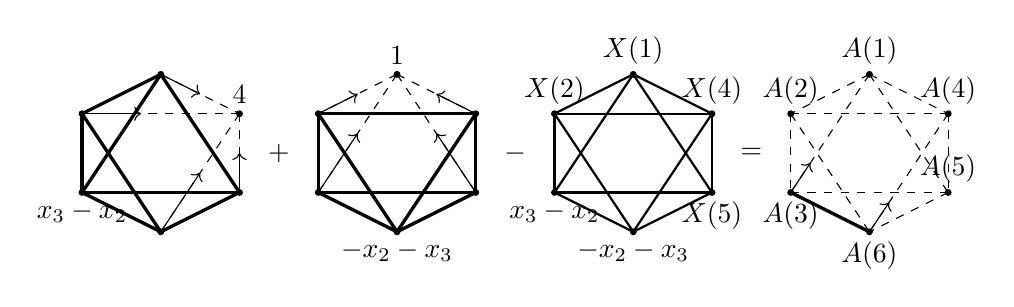
\begin{tikzpicture}
\begin{scope}[xscale=0.25, yscale=0.25]
\fill(0,4) circle (5pt);
\fill(-4,2) circle (5pt);
\fill(-4,-2) circle (5pt);
\fill(0,-4) circle (5pt);
\fill(4,-2) circle (5pt);
\fill(4,2) circle (5pt);

\draw[very thick] (0,4)--(-4,2);
\draw[very thick] (0,4)--(-4,-2);
\draw[very thick] (0,4)--(4,-2);
\draw[dashed] (0,4)--(4,2);
\draw[very thick] (-4,2)--(-4,-2);
\draw[very thick] (-4,2)--(0,-4);
\draw[dashed] (-4,2)--(4,2);
\draw[very thick] (-4,-2)--(4,-2);
\draw[very thick] (-4,-2)--(0,-4);
\draw[dashed] (4,2)--(4,-2);
\draw[dashed] (4,2)--(0,-4);
\draw[very thick] (4,-2)--(0,-4);

\draw[->] (-4,2)--(-1,2);
\draw[->] (0,4)--(2,3);
\draw[->] (4,-2)--(4,0);
\draw[->] (0,-4)--(2,-1);

\node at (6,0) {$+$};

\fill(12,4) circle (5pt);
\fill(8,2) circle (5pt);
\fill(8,-2) circle (5pt);
\fill(12,-4) circle (5pt);
\fill(16,-2) circle (5pt);
\fill(16,2) circle (5pt);

\draw[dashed] (12,4)--(8,2);
\draw[dashed] (12,4)--(8,-2);
\draw[dashed] (12,4)--(16,-2);
\draw[dashed] (12,4)--(16,2);
\draw[very thick] (8,2)--(8,-2);
\draw[very thick] (8,2)--(12,-4);
\draw[very thick] (8,2)--(16,2);
\draw[very thick] (8,-2)--(16,-2);
\draw[very thick] (8,-2)--(12,-4);
\draw[very thick] (16,2)--(16,-2);
\draw[very thick] (16,2)--(12,-4);
\draw[very thick] (16,-2)--(12,-4);

\draw[->] (8,2)--(10,3);
\draw[->] (8,-2)--(10,1);
\draw[->] (16,-2)--(14,1);
\draw[->] (16,2)--(14,3);

\node[above] at (12,4) {$1$};
\node[above] at (4,2) {$4$};
\node[below] at (12,-4) {$-x_{2}-x_{3}$};
\node[below] at (-4,-2) {$x_{3}-x_{2}$};


\node at (18,0) {$-$};

\fill(24,4) circle (5pt);
\node[above] at (24,4) {$X(1)$};
\fill(20,2) circle (5pt);
\node[above] at (20,2) {$X(2)$};
\fill(20,-2) circle (5pt);
\node[below] at (20,-2) {$x_{3}-x_{2}$};
\fill(24,-4) circle (5pt);
\node[below] at (24,-4) {$-x_{2}-x_{3}$};
\fill(28,-2) circle (5pt);
\node[below] at (28,-2) {$X(5)$};
\fill(28,2) circle (5pt);
\node[above] at (28,2) {$X(4)$};

\draw[thick] (24,4)--(20,2);
\draw[thick] (24,4)--(20,-2);
\draw[thick] (24,4)--(28,-2);
\draw[thick] (24,4)--(28,2);
\draw[thick] (20,2)--(20,-2);
\draw[thick] (20,2)--(24,-4);
\draw[thick] (20,2)--(28,2);
\draw[thick] (20,-2)--(28,-2);
\draw[thick] (20,-2)--(24,-4);
\draw[thick] (28,2)--(28,-2);
\draw[thick] (28,2)--(24,-4);
\draw[thick] (28,-2)--(24,-4);

\node at (30,0) {$=$};

%--+24

\fill(36,4) circle (5pt);
\fill(32,2) circle (5pt);
\fill(32,-2) circle (5pt);
\fill(36,-4) circle (5pt);
\fill(40,-2) circle (5pt);
\fill(40,2) circle (5pt);

\draw[dashed] (36,4)--(32,2);
\draw[dashed] (36,4)--(32,-2);
\draw[dashed] (36,4)--(40,-2);
\draw[dashed] (36,4)--(40,2);
\draw[dashed] (32,2)--(32,-2);
\draw[dashed] (32,2)--(36,-4);
\draw[dashed] (32,2)--(40,2);
\draw[dashed] (32,-2)--(40,-2);
\draw[very thick] (32,-2)--(36,-4);
\draw[dashed] (40,2)--(40,-2);
\draw[dashed] (40,2)--(36,-4);
\draw[dashed] (40,-2)--(36,-4);

\draw[->] (32,-2)--(33,-0.5);
\draw[->] (36,-4)--(37,-2.5);

\node[below] at (32,-2) {$A(3)$};
\node[below] at (36,-4) {$A(6)$};
\node[above] at (36, 4) {$A(1)$};
\node[above] at (32, 2) {$A(2)$};
\node[above] at (40, 2) {$A(4)$};
\node[above] at (40, -2) {$A(5)$};


\end{scope}
\end{tikzpicture}

\end{document}